        	\begin{question}{1217}{Trigonométrie}{1}{/}
				Dans un triangle rectangle, on cherche la relation qui relie un angle (différent de l'angle droit) avec les longueurs du côté adjacent à l'angle et de l'hypoténuse (le grand côté). A quoi est égal $\frac{adjacent}{hypotenuse}$?
            \end{question}
            \begin{reponses}
            	\item[false] $\sin(angle)$
            	\item[false] $\tan(angle)$
                \item[true] $\cos(angle)$
                \item[false] $angle$
            \end{reponses}
			%%%%%%%%%%%%%%%%%%%%%%%%%%%%%%%%%%%%%
        	\begin{question}{1217}{Trigonométrie}{1}{/}
				Dans un triangle rectangle, on cherche la relation qui relie un angle (différent de l'angle droit) avec les longueurs du côté opposé à l'angle et de l'hypoténuse (le grand côté). A quoi est égal $\frac{oppose}{hypotenuse}$?
            \end{question}
            \begin{reponses}
            	\item[true] $\sin(angle)$
            	\item[false] $\tan(angle)$
                \item[false] $\cos(angle)$
                \item[false] $angle$
            \end{reponses}
			%%%%%%%%%%%%%%%%%%%%%%%%%%%%%%%%%%%%%
        	\begin{question}{1217}{Trigonométrie}{1}{/}
				Dans un triangle rectangle, on cherche la relation qui relie un angle (différent de l'angle droit) avec les longueurs du côté adjacent à l'angle et du côté opposé à l'angle. A quoi est égal $\frac{oppose}{adjacent}$?
            \end{question}
            \begin{reponses}
            	\item[false] $\sin(angle)$
                \item[true] $\tan(angle)$
                \item[false] $\cos(angle)$
            	\item[false] $angle$
            \end{reponses}
			%%%%%%%%%%%%%%%%%%%%%%%%%%%%%%%%%%%%
        	\begin{question}{1217}{Trigonométrie}{1}{/}
				Dans un triangle rectangle, on cherche la relation qui relie un angle $\alpha$ (différent de l'angle droit) avec les longueurs du côté adjacent $AB$ à l'angle et de l'hypoténuse $AC$ (le grand côté). A quoi est égal $\frac{AB}{AC}$?
            \end{question}
            \begin{reponses}
            	\item[false] $\sin(\alpha)$
            	\item[false] $\tan(\alpha)$
                \item[true] $\cos(\alpha)$
                \item[false] $\alpha$
            \end{reponses}
			%%%%%%%%%%%%%%%%%%%%%%%%%%%%%%%%%%%%%
        	\begin{question}{1217}{Trigonométrie}{1}{/}
				Dans un triangle rectangle, on cherche la relation qui relie un angle $\alpha$ (différent de l'angle droit) avec les longueurs du côté $AB$ opposé à l'angle et de l'hypoténuse $AC$ (le grand côté). A quoi est égal $\frac{AB}{AC}$?
            \end{question}
            \begin{reponses}
            	\item[true] $\sin(\alpha)$
            	\item[false] $\tan(\alpha)$
                \item[false] $\cos(\alpha)$
                \item[false] $\alpha$
            \end{reponses}
			%%%%%%%%%%%%%%%%%%%%%%%%%%%%%%%%%%%%%
        	\begin{question}{1217}{Trigonométrie}{1}{/}
				Dans un triangle rectangle, on cherche la relation qui relie un angle $\alpha$ (différent de l'angle droit) avec les longueurs du côté $AB$ adjacent à l'angle et du côté $BC$ opposé à l'angle. A quoi est égal $\frac{BC}{AB}$?
            \end{question}
            \begin{reponses}
            	\item[false] $\sin(\alpha)$
                \item[true] $\tan(\alpha)$
                \item[false] $\cos(\alpha)$
            	\item[false] $\alpha$
            \end{reponses}
			%%%%%%%%%%%%%%%%%%%%%%%%%%%%%%%%%%%%
            \begin{question}{1217}{Trigonométrie}{2}{/}
                Que vaut l'angle $\hat{BAC}$?
                \begin{center}
                	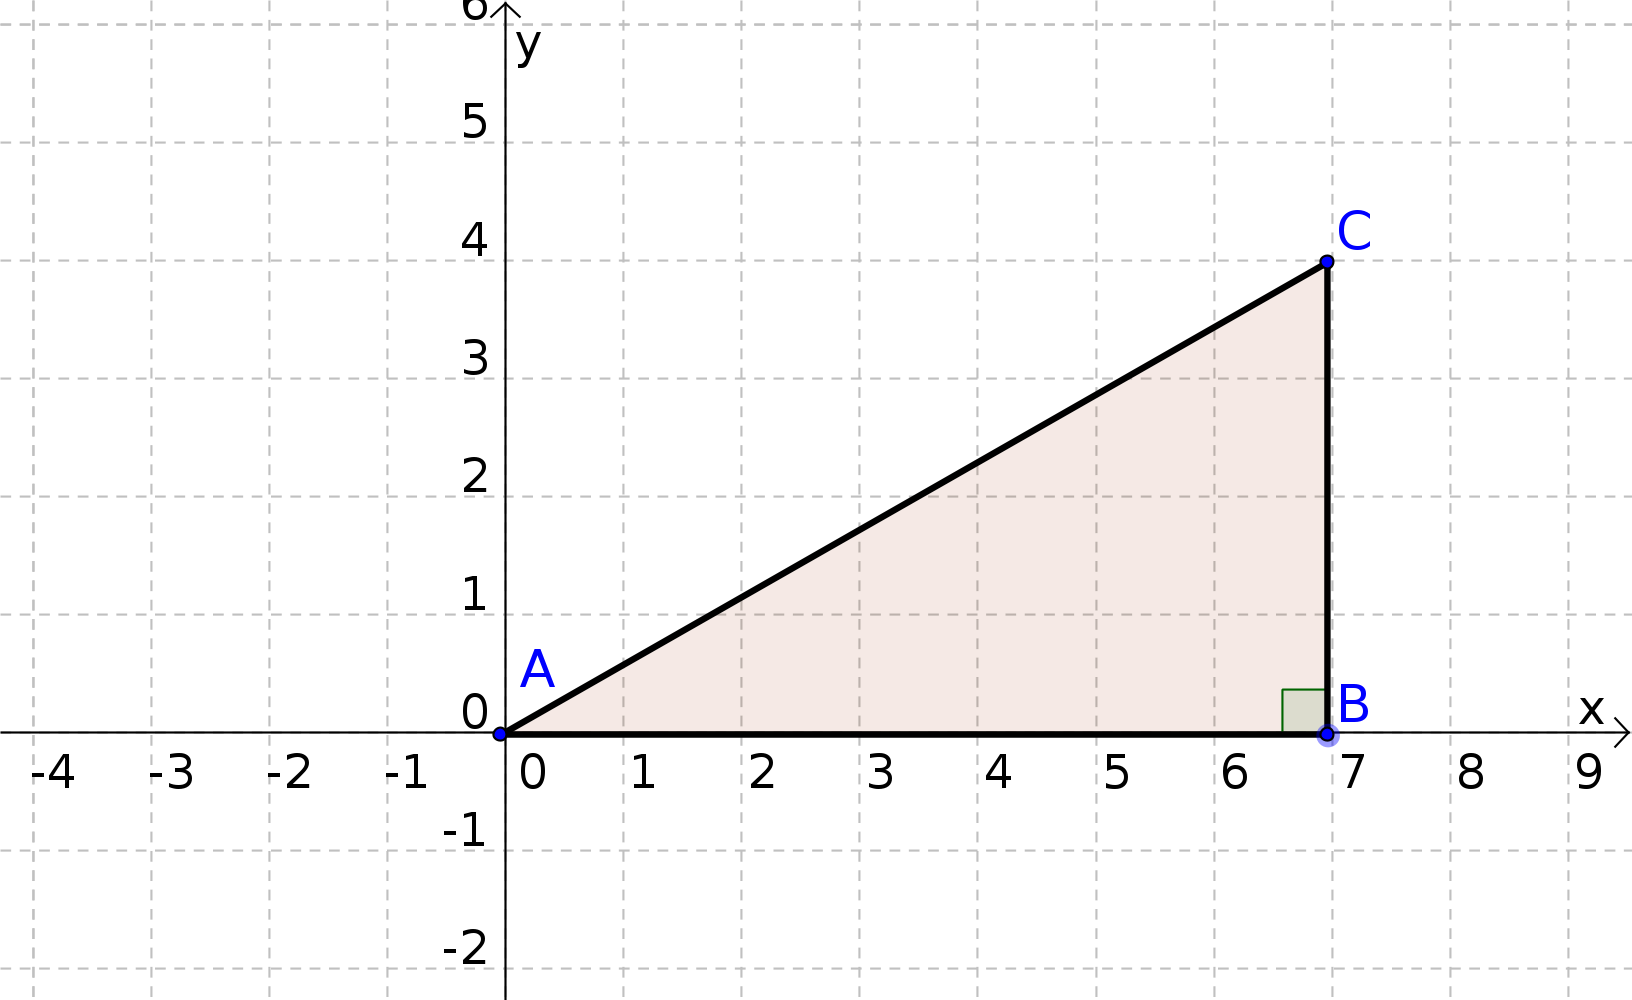
\includegraphics[width=0.5\textwidth]{Philippe/Figures_Philippe/trigo_1_1.png}
                \end{center}
            \end{question}
            \begin{reponses}
                \item[false] $\sin(4/7)$
                \item[true] $\arctan(4/7)$
                \item[false] $\tan(4/7)$
                \item[false] $\arcsin(4/7)$
            \end{reponses}
            %%%%%%%%%%%%%%%%%%%%%%%%%%%%%%%%%%%%%
